\documentclass{bioinfo}
\copyrightyear{2014}
\pubyear{2014}

\begin{document}
\firstpage{1}

\title[chipPCR]{chipPCR: an R Package to Pre-Process Amplification Curve Data}
\author[R\"odiger \textit{et~al.}]{Stefan R\"odiger\,$^{1}$\footnote{to whom correspondence should be addressed}, Micha\l{} Burdukiewicz\,$^{2}$ and Peter Schierack\,$^1$}
\address{$^{1}$Faculty of Natural Sciences, Brandenburg University of Technology 
Cottbus--Senftenberg, Senftenberg, Germany\\
$^{2}$Department of Genomics, Faculty of Biotechnology, University of 
Wroc\l{}aw, Wroc\l{}aw, Poland}

\history{Received on XXXXX; revised on XXXXX; accepted on XXXXX}

\editor{Associate Editor: XXXXXXX}

\maketitle

\begin{abstract}

\section{Motivation:}
Both the quantitative real-time polymerase chain reaction (qPCR) and quantitative 
isothermal amplification (qIA) are standard methods for nucleic acid 
quantification. Numerous real-time read-out technologies have been developed. Despite the growing interest in 
amplification-based techniques, there are only few tools for pre-processing of amplification data. 
However, a transparent  tool for precise control of raw data is indispensable in several scenarios, 
for example, during the development of new instruments.

\section{Results:}
$\emph{chipPCR}$ is an \textbf{R} package for the pre-processing and quality 
analysis of raw data of amplification curves. The package takes advantage of 
\textbf{R}'s \emph{S4} object model and offers an extensible environment. 
$\emph{chipPCR}$ contains tools for raw data exploration: normalization, 
baselining, imputation of missing values, a powerful wrapper for amplification 
curve smoothing and a function to detect the start and end of an amplification 
curve. The capabilities of the software are enhanced by the implementation of 
algorithms unavailable in \textbf{R}, such as a 5-point stencil for 
derivative interpolation. Simulation tools, statistical tests, plots for data 
quality management, amplification efficiency/quantification cycle calculation, 
and data sets from various qPCR and qIA experiments are part of the 
package. Core functionalities are integrated in GUIs 
(web-based and standalone \emph{shiny} applications), thus streamlining analysis 
and report generation.

\section{Availability:}
http://cran.r-project.org/web/packages/chipPCR\newline
Source code: https://github.com/michbur/chipPCR

\section{Contact:} \href{stefan.roediger@b-tu.de}{stefan.roediger@b-tu.de}

\section{Supplementary:} Supplementary data are available at Bioinformatics online.
\end{abstract}

\section{Introduction}

Quantitative polymerase chain reaction (qPCR) and quantitative isothermal 
amplification (qIA) are standard methods used for nucleic acid amplification. 
qPCR and qIA are used in real-time monitoring technologies, such as our 
previously reported VideoScan technology 
\citep{roediger_highly_2013,spiess_impact_2014}, microfluidics and point-of-care 
devices to quantify nucleic acids by specific curve parameters like the 
quantification point (Cq) \citep{pabinger_2014,rodiger_nucleic_2014}. The 
fundamental steps of amplification curve analysis are 1) raw data read-in, 2) 
pre-processing (e.g., noise reduction), 3) amplification curve processing (e.g., 
Cq calculation), 4) post-processing and 5) data export/report generation. 
Reliable data flow between all steps is a requirement for the proper 
optimization (e.g., the Taguchi method) of amplification reactions 
\citep{cobb_1994}. \textbf{R} is widely used in bioinformatics and an early 
adopter of novel technologies (e.g., digital PCR, NanoString nCounter Platform) 
\citep{waggott_2012,pabinger_2014}. Available \textbf{R} packages focus on the 
read-in and (post)-processing of data from commercial qPCR systems. \textbf{R} 
packages for the amplification analysis steps 1 and 3--5 cited above are 
available \citep{perkins_2012,gehlenborg_2013,mccall_2014,pabinger_2014}. 
However, \textbf{R} package for the pre-processing and quality 
analysis of raw data of amplification curves are unavailable. Pre-processing in most commercial 
cyclers is a black box, which restrains reproducible research 
\citep{Leeper_2014}. The development and optimization of equipment would benefit 
from the availability of a software capable of pre-processing raw data. 
Pre-processing algorithms remove stochastic errors and artefacts (Suppl. 
Sect.~2) and provide the means for raw data inspection and transformation in a 
format suitable for successive analysis steps (e.g., smoothing, imputation), 
data reduction (e.g., removal of invalid sets) and data quality management. 
Misinterpretations are more likely if arbitrary corrections are performed and a 
manual alteration is contradictory to reproducible research.

The $\emph{chipPCR}$ (``Lab-on-a-Chip'' \& PCR) package was 
developed to automatize pre-processing, analysis, visualization, and quality 
control of qPCR and qIA experiments. \textbf{R} enables sophisticated 
statistical and reproducible cross-platform analysis, and quick adaptation to 
changing experimental setups. Moreover, it is advantageous to set up workflows 
in an open environment, which offers GUIs, downstream analyses facilities, 
powerful data visualizations and report generation. The target audience 
encompasses developers and users who process raw data from commercial systems.

\section{Implementation}
\begin{methods}
We implemented the $\emph{chipPCR}$ package in the \textbf{R} software 
environment. $\emph{chipPCR}$ is a relative of the \emph{MBmca} 
\citep{roediger_RJ_2013}, the $\emph{RDML}$ \citep{blagodatskikh_2014}, and the 
\emph{dpcR} \citep{pabinger_2014} packages, but focusses on pre-processing of 
amplification curves. The package contains pre-processor functions (smoothing, 
imputation, background range detection, baseline correction and normalization), 
a single-blinded randomized rating function, quality analysis summary functions, 
an amplification efficiency function, an amplification curve simulator
and a report generation function (Suppl. Sect.~4). The supplemental material 
uses Donald Knuth's literate programming principle~\citep{Knuth1984} to 
conveniently present the source code. $\emph{chipPCR}$'s naming convention is 
\textit{period.separated} \citep{Baaaath_2012}. We use \textbf{R}'s object model 
\emph{S4} class system (see Supplement) to separate between interface and 
implementation. \emph{S4} classes require a higher effort than \emph{S3}, but 
assures better control on the object structure and the method dispatch. For fast 
running of codes in high-throughput applications, we avoided loops and left 
options for partially parallel computing usage (e.g., \textsl{smoother} 
function). $\emph{chipPCR}$ includes a set of classes for plotting. The output 
of our custom made plots is minimalistic, but many parameters can be adjusted 
directly or by the ellipse parameter.

We aim to make our software available for researchers not fluent in 
\textbf{R}. Therefore, we have implemented core functionality of our package in 
selected GUI technologies available in \textbf{R} \citep{rodiger_rkward_2012} as a
desktop application or web-based service. $\emph{chipPCR}$ offers the means to run 
the GUI applications as a service on a server without installing \textbf{R} (e.g., 
http://michbur.shinyapps.io/MFIaggr\_gui), on a local 
desktop (e.g., Fig.~S2,~S6), or as deployed from an external % Fig.~\ref{figure:browser}
source for a local \textbf{R} installation. The functions \textsl{AmpSim}, 
\textsl{th.cyc}, \textsl{bg.max} and \textsl{amptester} are part of online GUIs. 
We aimed to build monolithic systems to parse, pre-process and analyze 
amplification curve data in a combined work-flow. 

$\emph{chipPCR}$ relies solely on the native \textbf{R} 
workspace and dedicated \textbf{R} packages as default data import 
and export format \citep{perkins_2012,rodiger_rkward_2012,blagodatskikh_2014}. 
$\emph{chipPCR}$ presents \emph{S4} objects with tailored summary and plot 
methods. Since data sets are an essential element of reproducible research 
\citep{Leeper_2014}, we have included 22 data sets from commercial and 
experimental cyclers to this package.
\end{methods}

\section{Example: quality analysis}

\textsl{MFIaggr} is a versatile analytical and graphical tool for fast multiple 
comparison of cycle-dependent signal dispersion and distribution 
(Fig.~\ref{fig:01}). The continuous explanatory variable $x$ (cycle number) is 
used to describe its relationships to $n$ continuous predictor variables $y_i$ 
(fluorescence values), where $i \in \{1, ..., n\}$. Use cases include the 
comparison of independent reaction vessels or the analysis of replicate 
experiments (Suppl. Sect.~6). In particular, this function might be useful for 
quality management during the development of high-throughput technologies. An 
analysis via the \emph{shiny} \textsl{MFIaggr.gui} app is shown in Fig.~S7.

\begin{figure}[!tpb]%figure1
\centerline{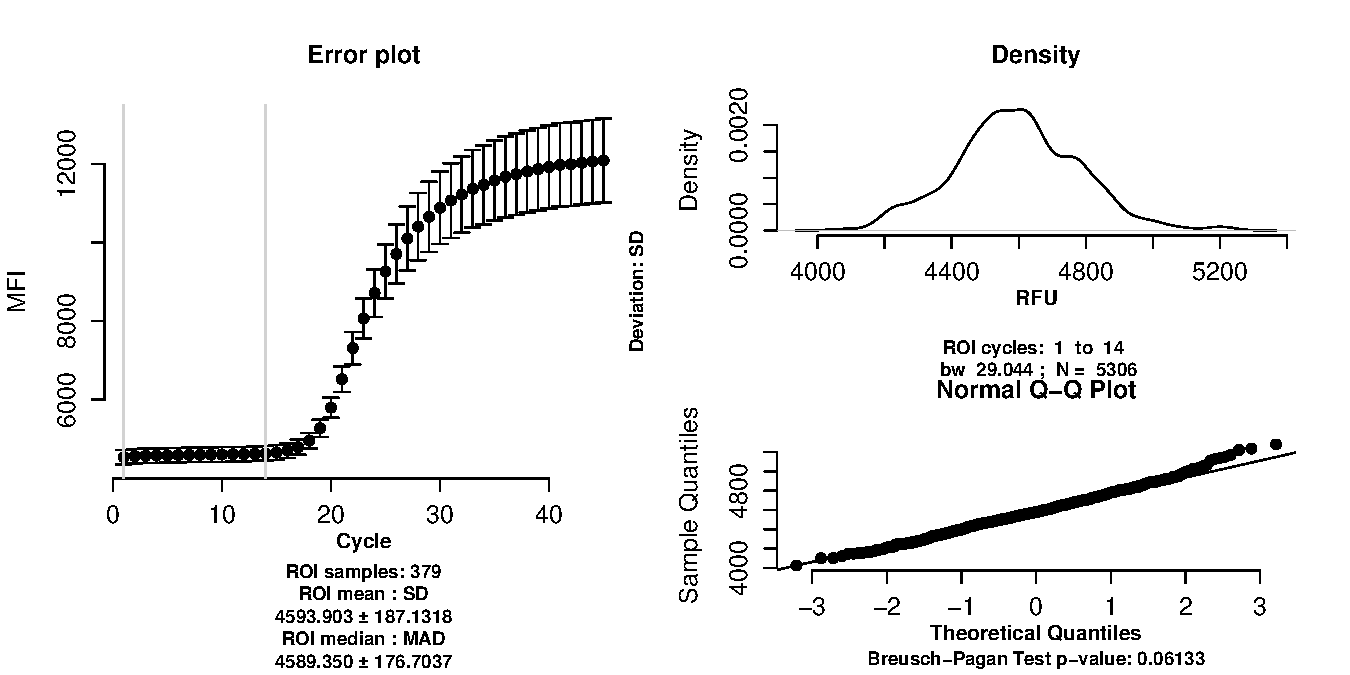
\includegraphics[width=8.7cm]{fig01.eps}}
\caption{\textsl{MFIaggr} plot for 379 replicate amplification curves. Cycles 1 to 14 were 
selected as region of interest (ROI) to analyze the 
cycle-dependent variance (left panel), the density plot (top-right 
panel) and quantile-quantile analysis (bottom-right panel), including a 
comprehensive statistical analysis as textual output (not shown). The plots 
indicate that the data of the background range are normal 
distributed. The heteroscedasticity is not significant.}\label{fig:01}
\end{figure}
\section{Results and Conclusions}
$\emph{chipPCR}$ is the first \textbf{R} package for the pre-processing and 
quality analysis of amplification curve raw data. In addition, we implemented 
standard methods for amplification curve processing. The $\emph{chipPCR}$ 
functions are embeddable in customized routines with other packages (see 
Suppl.), such as the \emph{RDML} and \emph{MBmca} packages. The modular package 
structure enables flexible data analysis adaptable to the requirements. Users can 
do estimations by hand. For example for Cq (SDM) estimation, solely the 
$\emph{chipPCR}$ functions \textsl{inder} and \textsl{smoother} are needed. 
\textsl{smoother} will be a method of smoothing in \textsl{inder}, and by 
putting data in the \textsl{bg} object with summary method \textsl{summary-der}, 
the user obtains the Cq. Through GUI's it should be easy for users without any 
\textbf{R} experience omitting a big limitation of qPCR and qIA \textbf{R} 
packages.


\section*{Acknowledgement}
\begin{methods}
Grateful thanks belong to the \textbf{R} community.

\paragraph{Funding\textcolon} This work was funded by the BMBF InnoProfile--Transfer--Projekt 03 IPT 611X.

\paragraph{Conflict of Interest\textcolon} none declared.
\end{methods}

\bibliographystyle{natbib}
%\bibliographystyle{achemnat}
%\bibliographystyle{plainnat}
%\bibliographystyle{abbrv}
%\bibliographystyle{bioinformatics}
%
%\bibliographystyle{plain}
%
\bibliography{Roediger_OxBio}
\end{document}
